%Advancments%
The evolution of AI in gaming, particularly through the development of AlphaGo,
AlphaGo Zero, and MuZero, highlights remarkable advancements in reinforcement
learning and artificial intelligence. AlphaGo, the pioneering model, combined
supervised learning and reinforcement learning to master the complex game of
Go, setting the stage for AI to exceed human capabilities in well-defined
strategic games. Building on, AlphaGo Zero eliminated the reliance on human
data, introducing a fully self-supervised approach that demonstrated greater
efficiency and performance by learning solely through self-play. MuZero took
this innovation further by generalizing beyond specific games like Go, Chess,
and Shogi, employing model-based reinforcement learning to predict dynamics
without explicitly knowing the rules of the environment. Completing on these
three models, here are some of the advancements that developed from them:
AlphaZero and MiniZero; and one of the most used in generating AI models,
Multi-agent models.
\subsection*{AlphaZero}
While AlphaGo Zero was an impressive feat, designed specifically to master the
ancient game of Go through self-play, AlphaZero developes it by generalizing
its learning framework to include multiple complex games: chess, shogi
(Japanese chess), and Go. The key advancement is in its ability to apply the
same algorithm across different games without requiring game-specific
adjustments. AlphaZero's neural network is trained through self-play,
predicting the move probabilities and game outcomes for various positions. This
prediction is then used to guide the MCTS, which explores potential future
moves and outcomes to determine the best action. Through iterative self-play
and continuous refinement of the neural network, AlphaZero efficiently learns
and improves its strategies across different games\cite{AD3}. Another
significant improvement is in AlphaZero’s generalized algorithm, is that it
does not need to be fine-tuned for each specific game. This was a departure
from AlphaGo Zero’s Go-specific architecture, making AlphaZero a more versatile
AI system.\\ AlphaZero's architecture integrates a single neural network that
evaluates both the best moves and the likelihood of winning from any given
position, streamlining the learning process by eliminating the need for
separate policy and value networks used in earlier systems. This innovation not
only enhances computational efficiency but also enables AlphaZero to adopt
unconventional and creative playing styles that diverge from established human
strategies.
\subsection*{MiniZero}
MiniZero is a a zero-knowledge learning framework that supports four
state-of-the-art algorithms, including AlphaZero, MuZero, Gumbel AlphaZero, and
Gumbel MuZero\cite{AD1}. Gumbel AlphaZero and Gumbel MuZero are variants of the
AlphaZero and MuZero algorithms that incorporate Gumbel noise into their
decision-making process to improve exploration and planning efficiency in
reinforcement learning tasks. Gumbel noise is a type of stochastic noise
sampled from the Gumbel distribution, commonly used in decision-making and
optimization problems.\\ MiniZero is a simplified version of the original
MuZero algorithm, which is designed to be have a more simplified architecture
reducing the complexity of the neural network used to model environment
dynamics, making it easier to implement and experiment with. This
simplification allows MiniZero to perform well in smaller environments with
fewer states and actions, offering faster training times and requiring fewer
computational power compared to MuZero.

\subsection*{Multi-agent models}
Multi-agent models in reinforcement learning (MARL) represent an extension of
traditional single-agent reinforcement learning. In these models, multiple
agents are simultaneously interacting, either competitively or cooperatively,
making decisions that impact both their own outcomes and those of other agents.
The complexity in multi-agent systems arises from the dynamic nature of the
environment, where the actions of each agent can alter the environment and the
states of other agents. Unlike in single-agent environments, where the agent
learns by interacting with a static world, multi-agent systems require agents
to learn not only from their direct experiences but also from the behaviors of
other agents, leading to a more complex learning process. Agents must adapt
their strategies based on what they perceive other agents are doing, and this
leads to problems such as strategic coordination, deception, negotiation, and
competitive dynamics. In competitive scenarios, agents might attempt to outwit
one another, while in cooperative scenarios, they must synchronize their
actions to achieve a common goal\cite{AD2}.\\ AlphaGo and AlphaGo Zero are not
designed to handle multi-agent environments. The core reason lies in their
foundational design, which assumes a single agent interacting with a static
environment. AlphaGo and AlphaGo Zero both rely on model-based reinforcement
learning and self-play, where a single agent learns by interacting with itself
or a fixed opponent, refining its strategy over time. However, these models are
not built to adapt to the dynamic nature of multi-agent environments, where the
state of the world constantly changes due to the actions of other agents. In
AlphaGo and AlphaGo Zero, the environment is well-defined, and the agent’s
objective is to optimize its moves based on a fixed set of rules. The agents in
these models do not need to account for the actions of other agents in
real-time or consider competing strategies, which are essential in multi-agent
systems. Additionally, AlphaGo and AlphaGo Zero are not designed to handle
cooperation or negotiation, which are key aspects of multi-agent
environments.\\ On the other hand, MuZero offers a more flexible framework that
can be adapted to multi-agent environments. Unlike AlphaGo and AlphaGo Zero,
MuZero operates by learning the dynamics of the environment through its
interactions, rather than relying on a fixed model of the world. This approach
allows MuZero to adapt to various types of environments, whether single-agent
or multi-agent, by learning to predict the consequences of actions without
needing explicit knowledge of the environment’s rules. The key advantage of
MuZero in multi-agent settings is its ability to plan and make decisions
without needing to model the entire system upfront. In multi-agent
environments, this ability becomes essential, as MuZero can dynamically adjust
its strategy based on the observed behavior of other agents. By learning not
just the immediate outcomes but also the strategic implications of others'
actions, MuZero can navigate both competitive and cooperative settings.
\begin{figure*}[t]
    \centering
    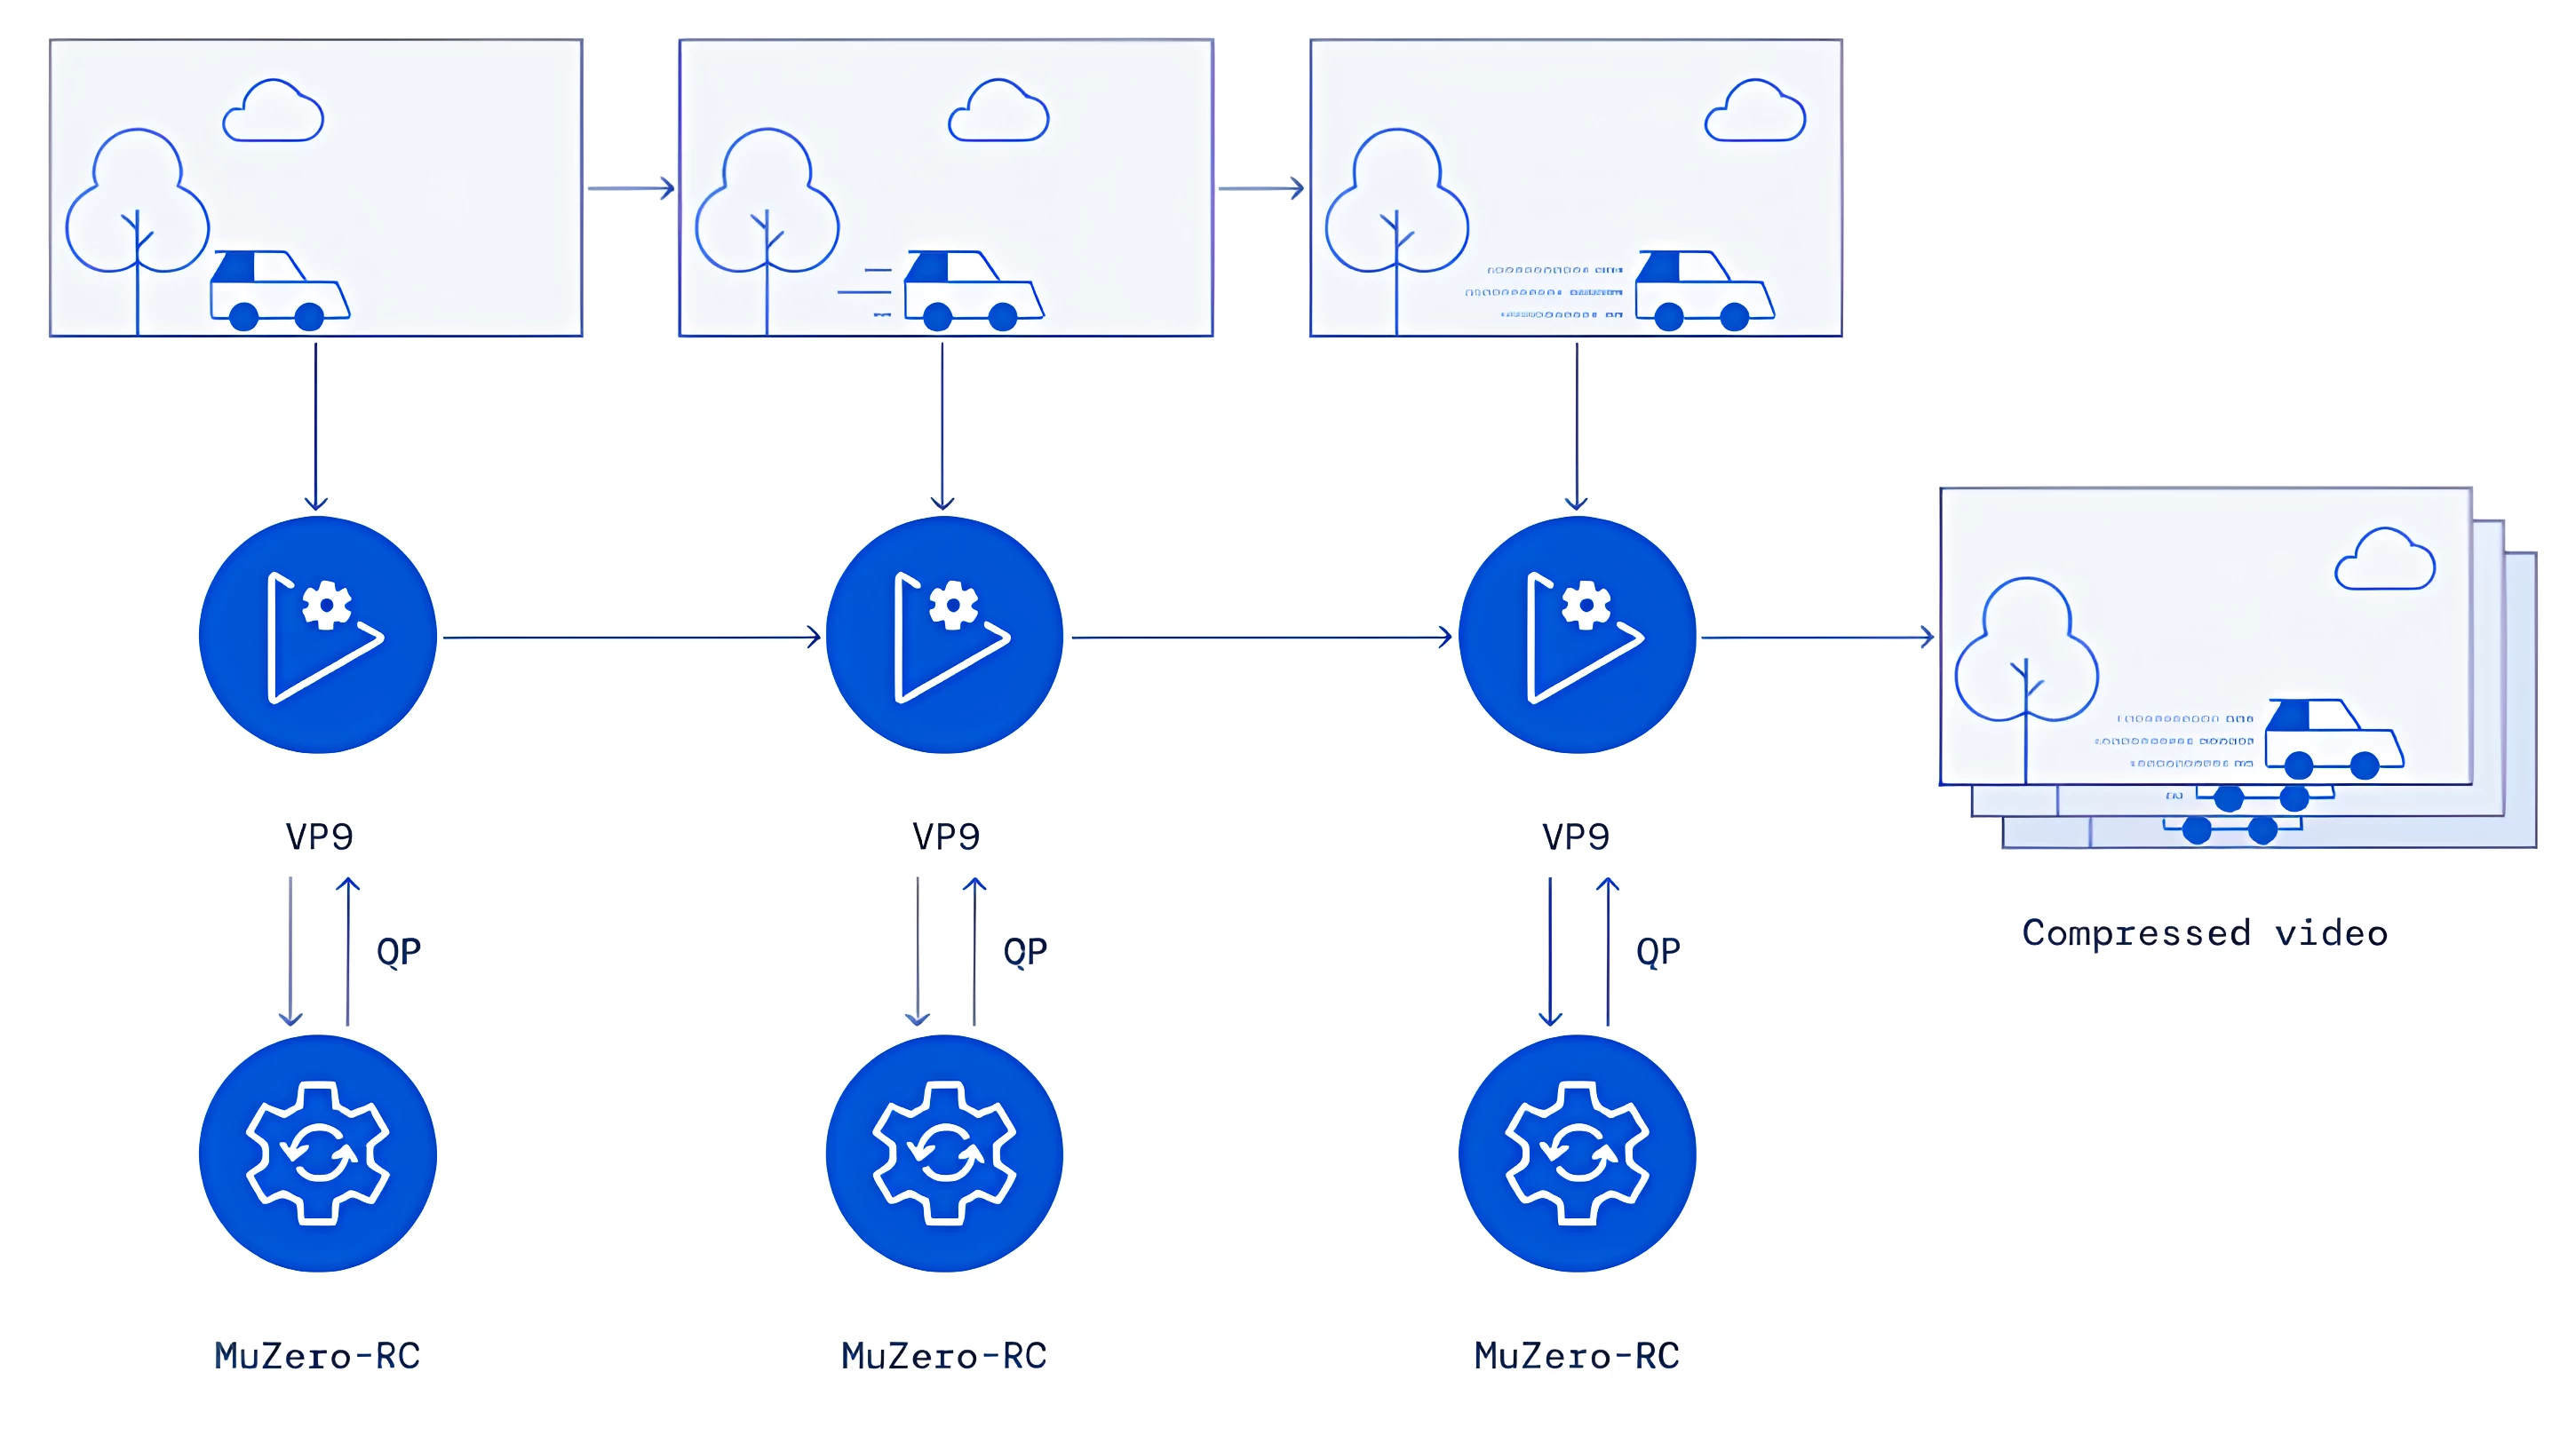
\includegraphics[width=0.7\textwidth]{sections/8Future Directions/MuZeroRC.png}
    \caption{MuZero Rate-Controller (MuZero-RC) optimizing the encoding process in video streaming.}
\end{figure*}